\documentclass[11pt,a4paper]{article}

\usepackage{graphicx}
\usepackage{sidecap}
\usepackage{mathtools}
%Om grotere integralen te krijgen
\usepackage{relsize}

%Andere breedte en lengthe van een document
\setlength{\textwidth}{6in} 
\addtolength{\hoffset}{-0.5in}
\setlength{\topmargin}{-0.2in}
\setlength{\textheight}{9in}

%Packages voor de figuren:
\usepackage{wrapfig}
\usepackage{caption}
\usepackage{subcaption}
%Kan er voor zorgen dat een figuur op de exacte plaats staat:
\usepackage{float}

\begin{document}
\begin{titlepage}
\title{\Huge Numerieke Wiskunde}
\author{Joni Allaert\\
		Ward Schodts\\
		}

\date{2013 - 2014}
\maketitle
\thispagestyle{empty}

\begin{center}


\includegraphics[scale=0.4]{KULzwart.png}

\end{center}
\begin{center}
\Large Professor Dr. ir. Marc Van Barel
\vfill
\end{center}
\end{titlepage}

\section{Deel 1: Numerieke integratie}
\subsection{Vast Deelinterval}
\subsubsection*{(a) Benadering van de integralen $\mathop{\mathlarger{\int\limits_{-1}^1e^xdx}}$ en  $\mathop{\mathlarger{\int\limits_{-5}^5\frac{1}{1+x^2}}}$}

\begin{figure}[H]

	\begin{subfigure}{0.5\textwidth}
	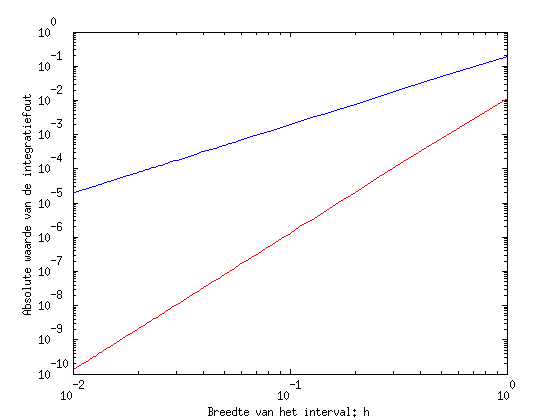
\includegraphics[width=\textwidth]{11a1.png}
	\caption*{$\int\limits_{-1}^1e^xdx$ met de trapeziumbenadering in het blauw en met de simpsonbenadering in het rood.}
	\end{subfigure}
	%Laat hier geen lijnen tussen anders komen ze niet meer horizontaal gelijk
	\begin{subfigure}{0.5\textwidth}
	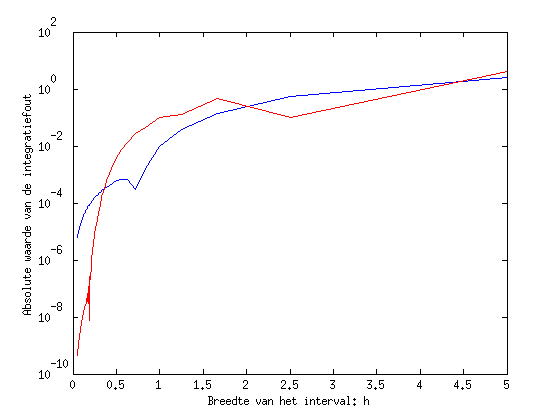
\includegraphics[width=\textwidth]{11a2.png}
	\caption*{$\int\limits_{-5}^5\frac{1}{1+x^2}$ met de trapeziumbenadering in het blauw en met de simpsonbenadering in het rood.}
	\end{subfigure}

\end{figure}

Om een duidelijk beeld te krijgen van de benaderingen, hebben we in het geval van de exponenti\"ele functie een loglog-plot genomen en voor de andere functie een semilogy-plot. Het doel was om de lijnen zo veel mogelijk te linearisren. In het geval van de tweede functie was dit echter niet mogelijk.

\subsubsection*{(b) De waardes $k$ in $O(h^k$) voor de integratieregels}

De fout die veroorzaakt wordt bij de trapeziumregel gedraagt zich als $O(h^2)$. De verklaring hiervoor is dat de integratiefout bij de trapeziumregel te schrijven is als \[ F_n = -\dfrac{(b-a)^3}{12n^2}f^{(2)}(\eta) \] voor een $\eta \in (a,b)$. De fout gedraagt zich bijgevolg als $O(n^{-2})$. Wat hetzelfde is als $O(h^2)$, per definitie van $h$.
\\
De fout veroorzaakt door de regel van Simpson gedraagt zich als $O(h^4)$. We kunnen immers de integratiefout bij de Simpsonregel schrijven als \[ F_n = -\dfrac{(b-a)^5}{180n^4}f^{(4)}(\eta) \] voor een $\eta \in (a,b)$. De fout gedraagt zich dan als $O(n^{-4})$. Dit is, per definitie van $h$, hetzelfde als $O(h^4)$.

\begin{figure}[H]

	\begin{subfigure}{0.5\textwidth}
	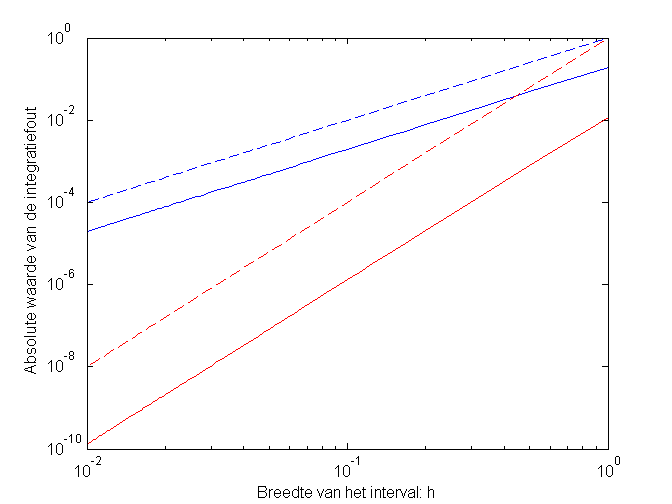
\includegraphics[width=\textwidth]{11b1.png}
	\caption*{$\int\limits_{-1}^1e^xdx$ het gedrag van de trapeziumbenadering met een blauwe stippellijn en het gedrag van de simpsonbenadering met een rode stippellijn.}
	\end{subfigure}
	%Laat hier geen lijnen tussen anders komen ze niet meer horizontaal gelijk
	\begin{subfigure}{0.5\textwidth}
	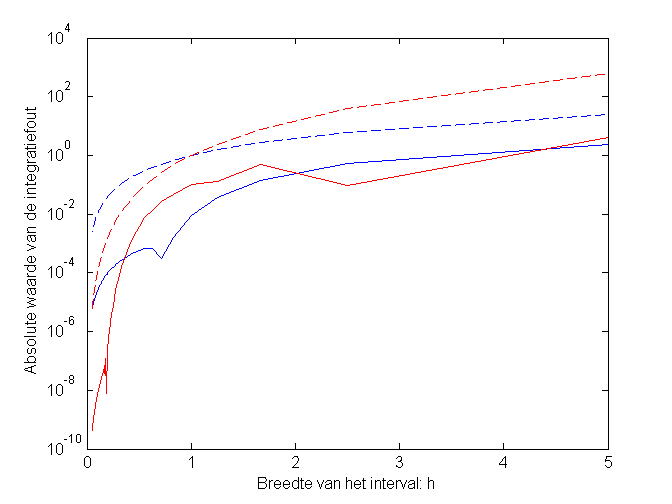
\includegraphics[width=\textwidth]{11b2.png}
	\caption*{$\int\limits_{-5}^5\frac{1}{1+x^2}$ het gedrag van de trapeziumbenadering met een blauwe stippellijn en het gedrag van de simpsonbenadering met een rode stippellijn.}
	\end{subfigure}

\end{figure}

\subsection{Adaptieve Routine}

\subsubsection*{(b) Het probleem bij $\mathop{\mathlarger{\int\limits_{-1}^1sin(2\pi x)^2dx}}$}

\subsubsection*{(c) Het probleem bij $\mathop{\mathlarger{\int\limits_{0}^1\frac{1}{\sqrt(x)}dx}}$}
Het probleem dat we hier krijgen is dat we de functie proberen te evalueren in punt waar hij niet gedefinieerd is. Namelijk het punt $x=0$. Hierdoor kijgen we een waarde $\infty$ voor zowel $I_1$ als $I_2$. Omdat er recursief altijd opnieuw wordt ge\"evalueerd wordt in $x=0$ dat telkens de waarde $\infty$ teruggeeft en bewerkingen hiermee ook $\infty$ teruggeven blijven we maar opnieuw recursief uitvoeren. Want de voorwaarde om met de recursie te stoppen: 
\begin{verbatim}
if abs(I1 - I2) < e
\end{verbatim}
is nooit voldaan dan.
\\
\\
De methode \verb|quad| lost dit probleem op met volgende code:
\begin{verbatim}
% Fudge endpoints to avoid infinities.
if ~isfinite(y(1))
    y(1) = f(a+eps(superiorfloat(a,b))*(b-a),varargin{:});
    fcnt = fcnt+1;
end
if ~isfinite(y(7))
    y(7) = f(b-eps(superiorfloat(a,b))*(b-a),varargin{:});
    fcnt = fcnt+1;
end
\end{verbatim}
\verb|quad| checkt dus of de eindpunten niet oneindig zijn en als dit zo is
\subsubsection*{(d) De uitvoeringstijd in functie van e }

\begin{figure}[H]
	\centering
	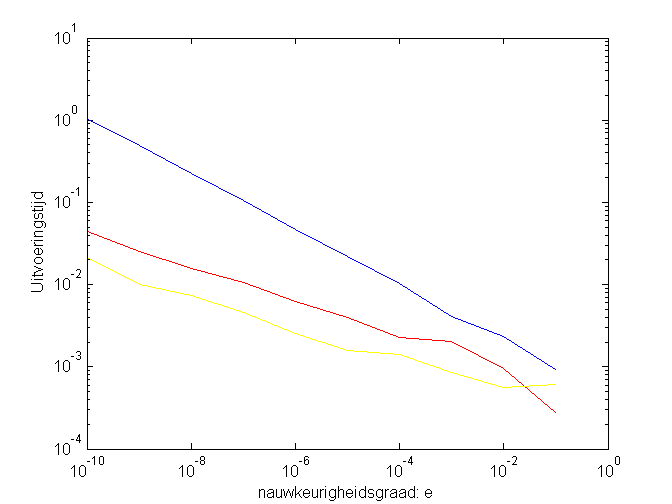
\includegraphics[width=0.7\textwidth]{12d1.png}
	\caption*{De uitvoeringstijden van trapezium, Simpson en quad in respectievelijke kleuren blauw, rood en geel}
	\end{figure}

\section{Deel 2: Kleinste kwadraten benadering van een functie}
\subsection{Veeltermbenadering in monomiaalbasis}
\subsubsection*{(d) De fout $||f-g||$ in functie van de graad}

\begin{figure}[H]
	\centering
	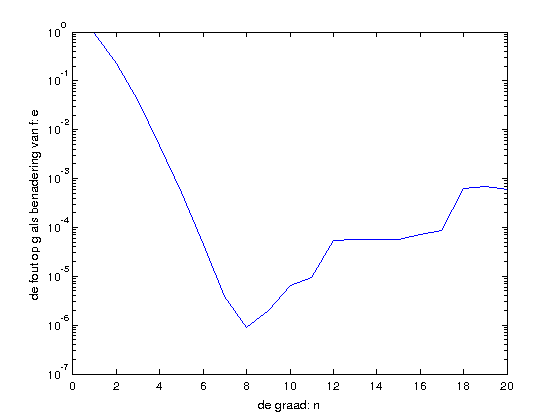
\includegraphics[width=0.7\textwidth]{22d1.png}
	\caption*{}
	\end{figure}
	
We hebben hier gekozen voor een semilogy-plot, omdat op deze figuur de lijnen het meest recht liepen.

\subsubsection*{(e) Benaderings- of abrekingsfout?}

Het eerste, dalende deel is te wijten aan de benaderingsfouten. Dit stuk daalt, want als de graad stijgt kunnen we de functie steeds beter en beter benaderen. Vanaf een bepaald moment (hier bij een fout van $10^{-6}$) nemen echter de afrondingsfouten de overhand en gaat de totale fout weer stijgen. Het stijgende tweede deel is dus te wijten aan afrondingsfouten.

\subsubsection*{(f) Convergentiesnelheid}

\begin{figure}[H]
	\centering
	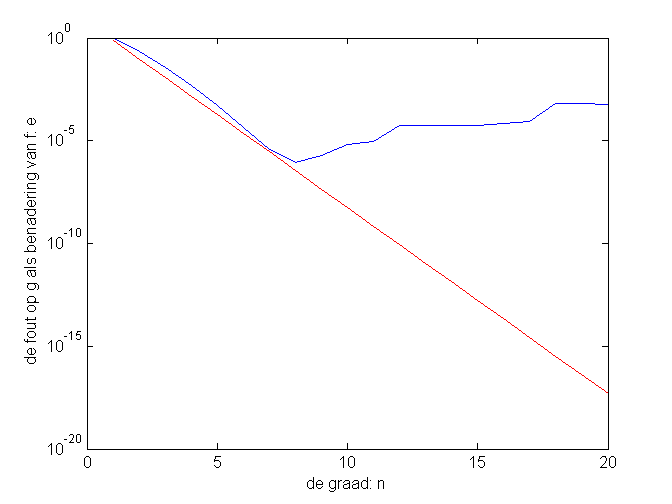
\includegraphics[width=0.7\textwidth]{22f1.png}
	\caption*{}
	\end{figure}
	
De convergentiesnelheid gedraagt zich als $O(8^{-n})$ met $n$ de graad van $g$.

\subsubsection*{(h) Perturbaties op A en b}

\begin{figure}[H]
	\centering
	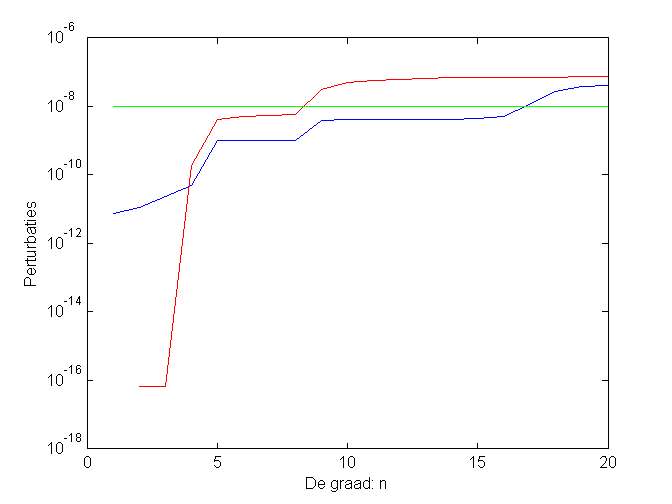
\includegraphics[width=0.7\textwidth]{22h1.png}
	\caption*{Perturbaties op A(rood), b(blauw)}
	\end{figure}

De groene lijn geeft aan waar $10^{-8}$. We kunnen dus duidelijk zien dat op veelvoud na $10^{-8}$ zijn. Met andere woorden ze zijn van grootorde $10^{-8}$.

\subsubsection*{(i) perturbatie op a}

\begin{figure}[H]
	\centering
	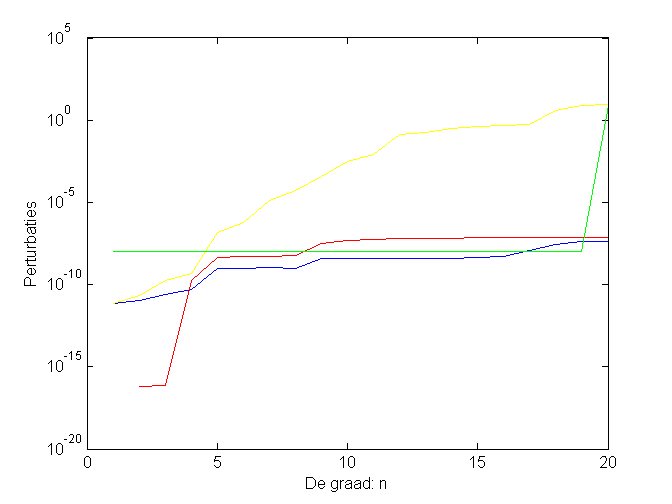
\includegraphics[width=0.7\textwidth]{22i1.png}
	\caption*{Perturbaties op a(geel) en tol vermenigvuldigd met het conditiegetal(groen) bijgevoegd}
	\end{figure}
	
\section{Tijdsbesteding}
\begin{center}
\begin{tabular}{ c || c }
Onderdeel & Tijdsbesteding\\
\hline
\hline
Doornemen opgave & 1u\\
\hline
Code deel 1 & 11u\\
\hline
Code deel 2 & 9u\\
\hline
Maken grafieken & 3u\\
\hline
Samenstellen verslag & 5u
\end{tabular}
\end{center}

\end{document}